% Adapted from figures/swat/SWaT_collection_campaign.pdf.
% Campaign: Goh et al., Section 4. Exclusion: internal report, p. 39.
% D-055: the full 449,919-timestamp attack period is split chronologically.
% The first 56,240 timestamps support training and validation; the later 393,679 form the test.
\documentclass[border=1pt]{standalone}
% Shared typography and palette for the three corrected SWaT context figures.
% Geometry is in millimetres; 140 mm fits the thesis text block at native scale.
\usepackage[T1]{fontenc}
\usepackage{tgheros}
\renewcommand{\familydefault}{\sfdefault}
\usepackage{tikz}
\usetikzlibrary{calc,patterns}
\definecolor{swatblue}{HTML}{0065BD}
\definecolor{swatlight}{HTML}{98C6EA}
\definecolor{swatgrey}{HTML}{666666}
\tikzset{every node/.style={font=\fontsize{8}{10}\selectfont},
  panel/.style={draw=black!30,fill=white,line width=0.4pt},
  stage/.style={draw=swatblue,fill=swatblue,text=white,align=center,
    minimum height=10mm,text width=19mm,inner sep=0.5mm},
  smalllabel/.style={font=\fontsize{7}{8.5}\selectfont,text=swatgrey}}

\begin{document}
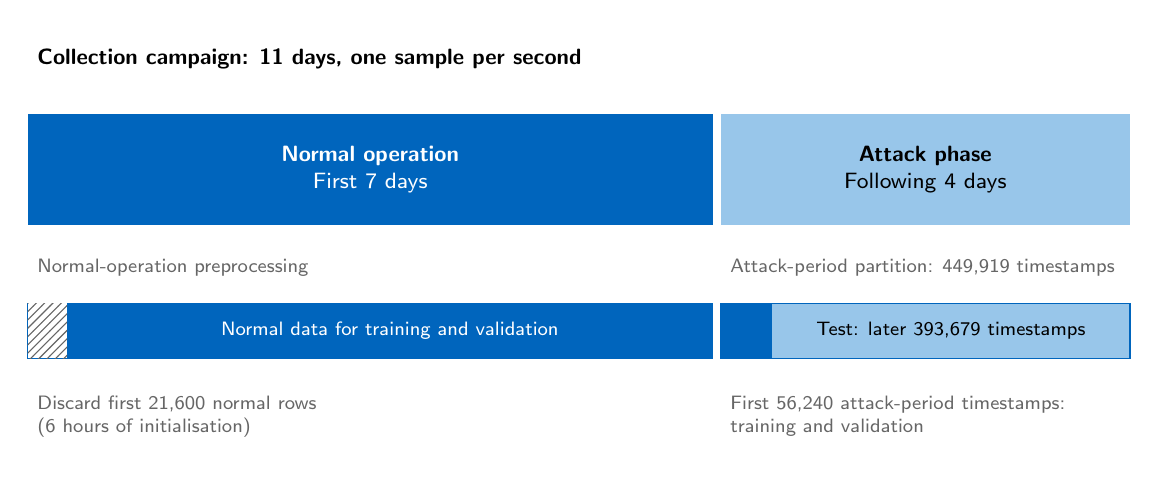
\begin{tikzpicture}[x=1mm,y=1mm]
  \path[use as bounding box] (0,0) rectangle (140,54);
  \node[anchor=west,font=\bfseries\fontsize{8}{10}\selectfont] at (0,50)
    {Collection campaign: 11 days, one sample per second};
  \fill[swatblue] (0,29) rectangle (87,43);
  \fill[swatlight] (88,29) rectangle (140,43);
  \node[align=center,text=white] at (43.5,36)
    {\textbf{Normal operation}\\First 7 days};
  \node[align=center] at (114,36)
    {\textbf{Attack phase}\\Following 4 days};
  \node[smalllabel,anchor=west] at (0,23.5) {Normal-operation preprocessing};
  \node[smalllabel,anchor=west] at (88,23.5) {Attack-period partition: 449,919 timestamps};
  \draw[draw=swatblue,fill=swatblue] (0,12) rectangle (87,19);
  \draw[draw=swatblue,fill=swatblue] (88,12) rectangle (94.5,19);
  \draw[draw=swatblue,fill=swatlight] (94.5,12) rectangle (140,19);
  \fill[white] (0,12) rectangle (5,19);
  \fill[pattern=north east lines,pattern color=swatgrey] (0,12) rectangle (5,19);
  \node[font=\fontsize{7}{8.5}\selectfont,text=white] at (46,15.5)
    {Normal data for training and validation};
  \node[font=\fontsize{7}{8.5}\selectfont,align=center] at (117.25,15.5)
    {Test: later 393,679 timestamps};
  \node[smalllabel,anchor=north west,align=left] at (0,8.5)
    {Discard first 21,600 normal rows\\(6 hours of initialisation)};
  \node[smalllabel,anchor=north west,align=left] at (88,8.5)
    {First 56,240 attack-period timestamps:\\training and validation};
\end{tikzpicture}
\end{document}
